\documentclass[a4paper,12pt]{article}
\usepackage{cmap}
\usepackage[T2A]{fontenc}
\usepackage[utf8]{inputenc}
\usepackage[english,russian]{babel}
\usepackage{listings}
\usepackage{amsmath}
\usepackage{float}
\usepackage{csquotes}
\usepackage{graphicx}
\usepackage{xcolor}
\usepackage{hyperref}
\usepackage{mathtools}

\renewcommand{\theequation}{\thesection.\arabic{equation}}


\author{Шерепа Никита}
\title{ThinkDSP. Лабораторная 2. Гармоники.}
\date{\today}

\graphicspath{{res/screenshots}}

\begin{document}%
	
	\maketitle
	
	\newpage \tableofcontents
	\newpage \listoffigures
	\newpage \lstlistoflistings
	
	\newpage
	
	\definecolor{dkgreen}{rgb}{0,0.6,0}
	\definecolor{gray}{rgb}{0.5,0.5,0.5}
	\definecolor{mauve}{rgb}{0.58,0,0.82}
	
	\lstset{
		language=Python,                 % выбор ЯП для подсветки 
		basicstyle=\small\sffamily, % размер и начертание шрифта для подсветки кода
		numbers=left,               % где поставить нумерацию строк (слева\справа)
		numberstyle=\tiny,           % размер шрифта для номеров строк
		stepnumber=1,                   % размер шага между двумя номерами строк
		numbersep=5pt,                % как далеко отстоят номера строк от подсвечиваемого кода
		aboveskip=3mm,
		belowskip=3mm,
		showstringspaces=false,
		columns=flexible,
		captionpos=b, 
		basicstyle={\small\ttfamily},
		numbers=left,
		numberstyle=\tiny\color{gray},
		keywordstyle=\color{blue},
		commentstyle=\color{mauve},
		stringstyle=\color{dkgreen},
		breaklines=true,
		breakatwhitespace=true,
		tabsize=3
	}

\section{Упражнение 2.2}

\begin{enumerate}
	
	\item \textbf{Задание}
	
	Пилообразный сигнал линейно нарастает от -1 до 1, а затем резко падает до -1 и повторяется.
	
	Напишите класс, называемый \textit{SawtoothSignal}, расширяющий \textit{signal} и предоставляющий \textit{evaluate} для оценки пилообразоного сигнала.
	
	Вычислите спектр пилообразного сигнала. Как соотносится его гармоническая структура с треугольным и прямоугольным сигналами?
	
	\item \textbf{Ход работы}
	
	Напишем класс \textit{SawtoothSignal}
	
	\begin{lstlisting}[caption=Класс SawtoothSignal]
		from thinkdsp import Sinusoid
		from thinkdsp import normalize, unbias
		import numpy as np
		
		class SawtoothSignal(Sinusoid):
			def evaluate(self, ts):
				cycles = self.freq * ts + self.offset / np.pi / 2
				frac, _ = np.modf(cycles)
				ys = normalize(unbias(frac), self.amp)
				return ys
	\end{lstlisting}
	
	Теперь сделаем пилообразный звук и прослушаем его
	\begin{lstlisting}[caption=Класс SawtoothSignal]
		sawtooth = SawtoothSignal().make_wave(duration=0.05, framerate=40000)
		sawtooth.make_audio()
	\end{lstlisting}
	
	Получился очень острый, высокий и неприятный звук
	Визуализируем его
	
	\begin{lstlisting}[caption=Визуализация звука]
		wave.plot()
	\end{lstlisting}
	\begin{figure}[H]
		\centering
		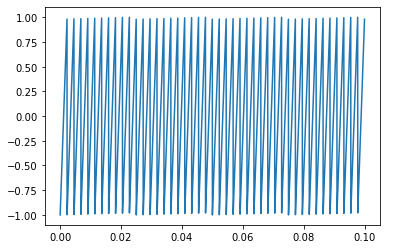
\includegraphics[width=0.75\textwidth]{2_1.png}
		\caption{Пилообразный звук}
		\label{fig:2.1}
	\end{figure}

	Теперь вычислим спектр пилообразного сигнала
	\begin{lstlisting}[caption=Спектр пилообразного сигнала]
		sawtooth.make_spectrum().plot()
	\end{lstlisting}
	\begin{figure}[H]
		\centering
		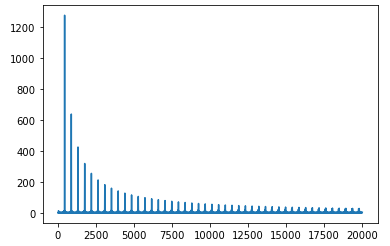
\includegraphics[width=0.75\textwidth]{2_2.png}
		\caption{Спектр пилообразного сигнала}
		\label{fig:2.2}
	\end{figure}
	
	
	Теперь составим прямоугольный сигнал и сравним его нармоническую структуру с гармонической структурой пилообразного сигнала
	\begin{lstlisting}[caption=Создание прямоугольного сигнала]
		from thinkdsp import SquareSignal
		
		sawtooth.make_spectrum().plot(color='red')
		square = SquareSignal(amp=0.5).make_wave(duration=0.1, framerate=40000)
		square.make_spectrum().plot()
	\end{lstlisting}
	\begin{figure}[H]
		\centering
		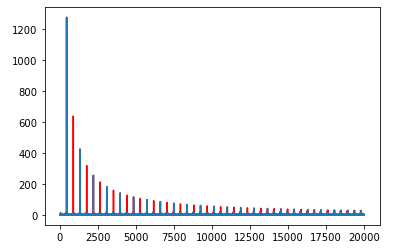
\includegraphics[width=0.75\textwidth]{2_3.png}
		\caption{Сравнение гармоник пилообразного сигнала (синий) и прямоугольного сигнала (красный)}
		\label{fig:2.3}
	\end{figure}
	
	Как видим, гармоники прямоугольного сигнала убывают аналогично гармоникам пилообразного сигнала. При этом у прямоугольного сигнала присутствуют как четные, так и нечетные гармоники.
	
	Теперь составим треугольный сигнал и сравним его нармоническую структуру с гармонической структурой пилообразного сигнала
	\begin{lstlisting}[caption=Создание треугольного сигнала]
		from thinkdsp import SquareSignal
		
		sawtooth.make_spectrum().plot(color='red')
		square = SquareSignal(amp=0.5).make_wave(duration=0.1, framerate=40000)
		square.make_spectrum().plot()
	\end{lstlisting}
	\begin{figure}[H]
		\centering
		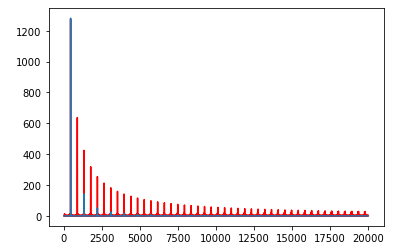
\includegraphics[width=0.75\textwidth]{2_4.png}
		\caption{Сравнение гармоник пилообразного сигнала (синий) и треугоьльного сигнала (красный)}
		\label{fig:2.4}
	\end{figure}

	Как видим, гармоники треугольного сигнала убывают не так резко по сравнению с гармоникам пилообразного сигнала. При этом у треугольного сигнала присутствуют как четные, так и нечетные гармоники.
	
	
\end{enumerate}

\newpage

\section{Упражнение 2.3}

\begin{enumerate}
	
	\item \textbf{Задание}
	
	Создайте прямоугольный сигнал 1100 Гц и вычислите \textit{wave} с выборками 10 000 кадров в секунду. Постройте спектр и убедитесь, что большинство гармоник "завернуты" из-за биений. Слышны ли последствия этого при проигрывании?
	
	\item \textbf{Ход работы}
	
	
	Создадим указанный сигнал и построим его спектр
	\begin{lstlisting}[caption=Создание сигнала и его спектра]
		square = SquareSignal(1100).make_wave(duration=0.5, framerate=10000)
		square.make_spectrum().plot()
	\end{lstlisting}
	\begin{figure}[H]
		\centering
		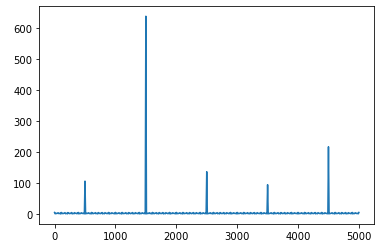
\includegraphics[width=0.75\textwidth]{3_1.png}
		\caption{Спектр созданного сигнала}
		\label{fig:3.1}
	\end{figure}
	Основная грамоника - 1100 Гц
	Первая гармоника - 3300 Гц
	Вторая гармоника - 4500 Гц, хотя должна быть на 5500 Гц
	Третья гармоника - 2300 Гц, хотя должна быть на 7700 Гц
	
	Теперь прослушаем получившийся сигнал 
	\begin{lstlisting}[caption=Прослушивание сигнала]
		square.make_audio()
	\end{lstlisting}
	
	Теперь как раз можно услышать эти сместившиеся гармоники.
	Теперь создадим сигнал с часотой 300 Гц и прослушаем.
	
	\begin{lstlisting}[caption=Создание сигнала с частотой 300 Гц и его прослушивание]
		from thinkdsp import SinSignal
		
		SinSignal(300).make_wave(duration=0.1, framerate=10000).make_audio()
	\end{lstlisting}
	
	Разница есть. Частоту можно отчетливо прослушать.
	
\end{enumerate}

\newpage

\section{Упражнение 2.4}

\begin{enumerate}
	
	\item \textbf{Задание}
	
	Возьмите объект \textit{Spectrum} и распечатайте несколько первых значений \textit{spectrum.fs}. Убедитесь, что они начинаются с нуля, то есть \textit{Spectrum.hs[0]} - амплитуда компоненты с частотой 0. Но что это значит?
	
	Проведите такой эксперимент:
	\begin{enumerate}
		\item Создайте треугольный сигнал с частотой 440 Гц и \textit{wave} длительностью 0.01 секунд. Распечатайте сигнал
		
		\item Создайте объект \textit{Spectrum} и распечатайте \textit{Spectrum.hs[0]}. Каковы амплитуда и фаза этого компонента?
		
		\item Установите \textit{Spectrum.hs[0]} = 100. Как эта операция повлияет на сигнал? Подсказка: \textit{Spectrum} дает метод, называемый \textit{make\_wave}, вычисляющий \textit{wave}, соответсвущий \textit{Spectrum}.
	\end{enumerate}
	
	\item \textbf{Ход работы}
	
	\begin{enumerate}
		\item Создадим треугольный сигнал и распечатаем его.
		
		\begin{lstlisting}[caption=Создание треугольного сигнала]
			triangle = TriangleSignal(440).make_wave(duration=0.01)
			triangle.plot()
		\end{lstlisting}
		\begin{figure}[H]
			\centering
			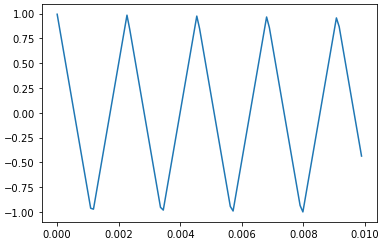
\includegraphics[width=0.75\textwidth]{4_1.png}
			\caption{Спектр созданного сигнала}
			\label{fig:4.1}
		\end{figure}
	
		\item Теперь выведем первый элемент спектра
		\begin{lstlisting}[caption=Первый элемент спектра]
			spectrum = triangle.make_spectrum()
			spectrum.hs[0]
			
			(1.0436096431476471e-14+0j)
		\end{lstlisting}	
	
		Получили комплексное число
		
		Если добавить в компонент нулевой частоты какое-то число - добавиться вертикальное смещение спектра
		
		\item Установим \textit{Spectrum} = 100
		\begin{lstlisting}[caption=Первый элемент спектра]
			spectrum.hs[0] = 100
			triangle.plot(color='red')
			spectrum.make_wave().plot()
		\end{lstlisting}
		\begin{figure}[H]
			\centering
			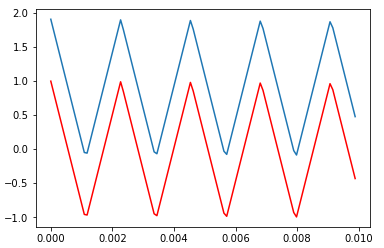
\includegraphics[width=0.75\textwidth]{4_2.png}
			\caption{Синий - первоначальный \textit{Spectrum.hs[0]}. Красный - \textit{Spectrum.hs[0]} = 100}
			\label{fig:4.2}
		\end{figure}
		Видим, что спектр сместился по вертикали относительно своего первоначального положения (красный график)
		
	\end{enumerate}
	
\end{enumerate}

\newpage

\section{Упражнение 2.5}

\begin{enumerate}
	
	\item \textbf{Задание}
	
	Напишите функцию, принимающую \textit{Spectrum} как параметр и изменяющую его делением каждого элемента \textit{hs} на соответсвующую частоту из \text{fs}. Подсказка: поскольку деление на ноль не определено, надо задать \textit{Spectrum.hs[0]} = 0.
	
	Проверье эту функцию, используя прямоугольный, треугольный или пилообразный сигналы:
	
	\begin{enumerate}
		
		\item Вычислите \textit{Spectrum} и распечатайте его
		
		\item Измените \textit{Spectrum}, вновь используя свою функцию, и распечатайте его
		
		\item Используйте \textit{Spectrum.make\_wave}, чтобы сделать \textit{wave} из измененного \textit{Spectrum}, и прослушайте его. Как эта операция повлияла на сигнал?
		
	\end{enumerate}
	
	\item \textbf{Ход работы}
	
	Напишем функцию для изменения спектра
	\begin{lstlisting}[caption=Функция для изменения спектра]
		def filter_spectrum(spectrum):
			spectrum.hs[1:] /= spectrum.fs[1:]
			spectrum.hs[0] = 0
	\end{lstlisting}
	
	Теперь вычислим первоначальный спектр и прослушаем
	\begin{lstlisting}[caption=Вычисление первоначального спектра и его прослушивание]
		wave = TriangleSignal(freq=440).make_wave(duration=0.5)
		wave.make_audio()
	\end{lstlisting}
	Звучит как гудок в телефоне
	
	Теперь, используя написанную функцию, изменим спектр
	\begin{lstlisting}[caption=Изменение спектра и визуализация результата]
		spectrum = wave.make_spectrum()
		spectrum.plot(high=10000, color='red')
		filter_spectrum(spectrum)
		spectrum.scale(440)
		spectrum.plot(high=10000)
	\end{lstlisting}
	\begin{figure}[H]
		\centering
		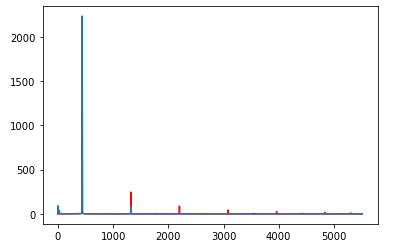
\includegraphics[width=0.75\textwidth]{5_1.png}
		\caption{Измененный спектр}
		\label{fig:5.1}
	\end{figure}
	
	И прослушаем получившийся результат
	\begin{lstlisting}[caption=Всопроизведение отфильтрованного спектра]
		filtered = spectrum.make_wave()
		filtered.make_audio()
	\end{lstlisting}

	Звук стал более глухой. По графику видно, что измененный спектр подавляет низкие гармоники исходного спектра и тем самым фильтрует низкие частоты.
	
\end{enumerate}

\newpage

\section{Упражнение 2.6}

\begin{enumerate}
	
	\item \textbf{Задание}
	
	У треугольных и прямоугольных сигналов есть только нечетные гармоники; в пилообразном сигнале есть и четные, и нечетные гармоники. Гармоники прямоугльных и пилообразных сигналов уменьшаются пропорционально \textit{1/f}; гамоники треугольных сигналов - пропорционально \textit{\(1/f^2\)}. Можно ли найти сигнал, состоящий из четных и нечетных гармоник, спадающих пропорционально \textit{\(1/f^2\)}?
	
	Подсказка: для этого есть два способа. 
	\begin{enumerate}
		
		\item Можно собрать желаемый сигнал из синусоид
		
		\item Можно взять сигнал со спектром, похожим на необходимый, и изменять его параметры
		
		
	\end{enumerate}
	
	\item \textbf{Ход работы}
	
	Создадим пилообразный спектр и визуализируем его
	\begin{lstlisting}[caption=Изменение спектра и визуализация результата]
		freq = 500
		signal = SawtoothSignal(freq=freq)
		wave = signal.make_wave(duration=0.5, framerate=20000)
		wave.make_audio()
		spectrum = wave.make_spectrum()
		spectrum.plot()
	\end{lstlisting}
	\begin{figure}[H]
		\centering
		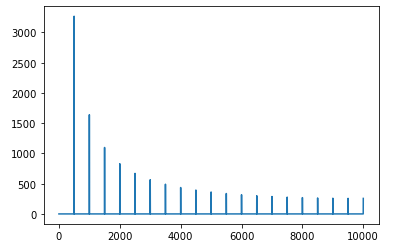
\includegraphics[width=0.75\textwidth]{6_1.png}
		\caption{Пилообразный спектр}
		\label{fig:6.1}
	\end{figure}

	Теперь воспользуемся функцией из прошлого упражнения, изменим полученный спектр и сравним результаты
		\begin{lstlisting}[caption=Изменеие спектра]
		spectrum.plot(color='red')
		filter_spectrum(spectrum)
		spectrum.scale(freq)
		spectrum.plot()
	\end{lstlisting}
	\begin{figure}[H]
		\centering
		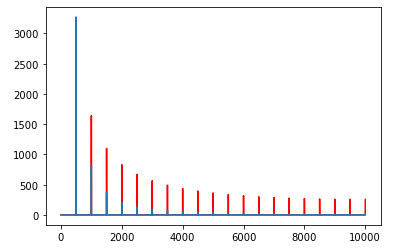
\includegraphics[width=0.75\textwidth]{6_2.png}
		\caption{Сравнение начального спектра и измененного спектра}
		\label{fig:6.2}
	\end{figure}
	
	Как видим, теперь гармоники получились схожими. Они спадают пропорционально \textit{\(1/f^2\)}
		
	Теперь помотрим, как выглядит получившийся результат
	\begin{lstlisting}[caption=Получившийся результат]
		wave.segment(duration=0.01).plot()
	\end{lstlisting}
	\begin{figure}[H]
		\centering
		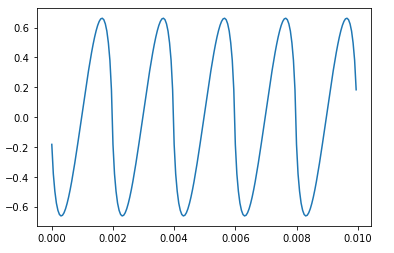
\includegraphics[width=0.75\textwidth]{6_3.png}
		\caption{Получившийся результат}
		\label{fig:6.2}
	\end{figure}

	Видим, что звук похож на синусоиду.
	
\end{enumerate}

\newpage

\section{Вывод}
В результате выполнения лабораторной работы получены навыки обработки пилообразных, прямоугольных, треугольных сигналов и их гармоник. Также в данной работе мы ознакомились с явлением смещения гармоник в цифровой обработке сигналов.

\end{document}